\documentclass[conference]{IEEEtran}
\IEEEoverridecommandlockouts
\usepackage{cite}
\usepackage{amsmath,amssymb,amsfonts}
\usepackage{graphicx}
\usepackage{textcomp}
\usepackage{xcolor}
\usepackage{booktabs}
\usepackage{array}
\usepackage[hidelinks]{hyperref}
\def\BibTeX{{\rm B\kern-.05em{\sc i\kern-.025em b}\kern-.08em T\kern-.1667em\lower.7ex\hbox{E}\kern-.125emX}}

\begin{document}

\title{From Verification to Forecasting:\\ Monitoring Official Crime Trends in Bangladesh}

\author{
\IEEEauthorblockN{Ifaz Ahmed Chowdhury}
\IEEEauthorblockA{\textit{Dept.\ of CSE}\\
\textit{BUBT}\\
Dhaka, Bangladesh\\
{\footnotesize 19202103469@cse.bubt.edu.bd}}
\and
\IEEEauthorblockN{Jubair Ahmed}
\IEEEauthorblockA{\textit{Dept.\ of CSE}\\
\textit{BUBT}\\
Dhaka, Bangladesh\\
{\footnotesize 22234103202@cse.bubt.edu.bd}}
\and
\IEEEauthorblockN{Sakib Abdullah}
\IEEEauthorblockA{\textit{Dept.\ of CSE}\\
\textit{BUBT}\\
Dhaka, Bangladesh\\
{\footnotesize 22234203230@cse.bubt.edu.bd}}
\and
\IEEEauthorblockN{Md.\ Imran Hasan Shanto}
\IEEEauthorblockA{\textit{Dept.\ of CSE}\\
\textit{BUBT}\\
Dhaka, Bangladesh\\
{\footnotesize 22234103400@cse.bubt.edu.bd}}
}

\maketitle

\begin{abstract}
Bangladesh Police Headquarters (PHQ) publishes monthly crime statistics, yet these series have not
been used as the basis for a validated, continuously updated forecasting system. We build one on
PHQ data spanning January 2019 to April 2026 (88 months, 17 reporting units, 15 crime types).
Three requirements shape the design: every value is traceable to the original signed PHQ
statements; forecast accuracy is measured strictly out of sample; and the pipeline is engineered to
run each month as new data is released. The dataset passes a five-step audit against 22 source
documents---all 88 months reconcile internally, the six complete years are cross-checked against
PHQ's independently printed annual pages, and a 429-cell re-audit of the most recent window matches
the source exactly. We evaluate seven standard forecasting models and their ensemble, trained on
data through April 2025 and tested against figures PHQ released afterward. In a single-origin
back-test of national Total Cases the forecast was 98.9\% accurate at 1 month, 97.8\% at 3 months,
92.8\% at 6 months, and 86.1\% at 12 months; a separate rolling-origin validation, averaged over the
stable crime categories, ranged from 94.7\% (1 month) to 89.9\% (12 months). The two are measured
differently and reported separately, and the ensemble was the most reliable model. An
interpretability layer reports the months and categories that drive forecast error, and a deployed
monitoring application ingests each new month, re-scores the prior forecast, and retrains. A
Transformer baseline did not improve on the classical models at this sample size. Forward
projections are presented as planning scenarios with no accuracy claim. The system forecasts
\emph{reported} crime counts; it does not estimate unreported crime or attribute causes to observed
changes.
\end{abstract}

\begin{IEEEkeywords}
reported-crime forecasting, rolling-origin validation, backtesting, MAPE, time-series,
Bangladesh, Police Headquarters, source verification, operational monitoring, explainability
\end{IEEEkeywords}

\section{Introduction}
Official crime statistics inform the allocation of policing resources, budget planning, and
public-safety policy. In Bangladesh, Police Headquarters (PHQ) releases a national crime report
each month. Reliable short- and medium-term forecasts of these figures would let planners act in
anticipation rather than only in response.

We restrict the target deliberately. The system forecasts \emph{reported} crime---incidents
recorded by police and published in the official PHQ statements---which is a subset of all crime,
since not every incident is reported. It does not forecast unreported crime, and it does not
predict offences by individuals or at specific locations; it forecasts the official monthly counts
and tracks their movement over time.

Three commitments separate this work from prior crime-forecasting studies on Bangladeshi data. The
first is provenance: every value is traceable to a signed PHQ document. The second is evaluation
discipline: accuracy is measured strictly out of sample (Section~\ref{sec:terms}) and then
confirmed by comparing a forecast fixed at a past date against months PHQ released only afterward.
The third is operational continuity: the forecasting logic is embedded in a monitoring application
that updates as each month arrives. We attach no accuracy claim to the forward scenario projection.

\subsection{Contributions}
This paper contributes:
\begin{enumerate}
  \item \textbf{A source-verified PHQ dataset} for January 2019 to April 2026, traced to the signed
        PHQ statements and checked by a five-step audit against 22 source documents: all 88 months
        reconcile internally, the six complete years (2019--2024) are cross-checked against PHQ's
        independently printed annual summary pages, and a 429-cell re-audit of the recent window
        matches the source exactly.
  \item \textbf{A leakage-free evaluation framework} combining rolling-origin validation with
        post-release back-testing. We train only on data up to April 2025, forecast 1, 3, 6, and 12
        months ahead, and compare against the real PHQ numbers released afterward.
  \item \textbf{An interpretability layer} that identifies which inputs the model relies on and
        which crime types are easy or hard to forecast.
  \item \textbf{A deployable monitoring application} that adds each new month, automatically
        re-checks the previous forecast, retrains, and watches for drift.
\end{enumerate}

\section{Related Work}
\subsection{Crime Forecasting in Bangladesh}
A few studies have applied machine learning to Bangladesh crime data. Awal et al.~\cite{awal2016}
used linear regression to forecast crime trends from Bangladesh Police records. Biswas and
Basak~\cite{biswas2019} extended this at an IEEE conference with polynomial and random-forest
regression on PHQ website data through 2018. Nahid~\cite{nahid2021} applied Random Forest, MLP,
and Decision Tree classifiers to PHQ data for five police units. Shohan et al.~\cite{shohan2022}
worked on a different problem, classifying incident-level crime from newspaper articles.

We examined what these studies documented. Biswas and Basak~\cite{biswas2019} describe
training their regression models on a training set and then forecasting on a separate test set
and comparing with the actual values, that is, a single fixed train--test split rather than a
time-series protocol that rolls forward month by month. Across these studies, after researching
the published papers, \emph{we have not seen documented evidence} of three things that our work
adds:
\begin{itemize}
  \item a source-verification audit that checks each number against the original PHQ documents;
  \item post-release back-testing, where a forecast made at a fixed past date is later compared
        against months that were published only afterward;
  \item an explainability layer that shows which crime types drive the forecast error.
\end{itemize}
We make this claim narrowly: not that these studies lack value, but that their published text does
not document these specific safeguards, which our work supplies.

\subsection{Forecasting Methods and Validation}
Testing a forecast on data it has already seen gives a falsely high score. Tashman~\cite{tashman2000}
reviews out-of-sample testing and recommends rolling-origin evaluation instead of a single split.
Bergmeir and Ben\'itez~\cite{bergmeir2012} show that rolling-origin protocols give more reliable
error estimates than random splits, which can leak future information. For measuring error,
Hyndman and Koehler~\cite{hyndman2006} analyse percentage- and scale-based measures and propose
the mean absolute scaled error (MASE); we report MAPE, WAPE, sMAPE, MAE, RMSE, and a seasonal
MASE. Classical models remain strong on short monthly data: the ARIMA/SARIMA
family~\cite{boxjenkins2015}, exponential smoothing (ETS)~\cite{hyndman2002ets}, and the Theta
method~\cite{assimakopoulos2000theta}, whose strength on monthly series was shown in the M3
competition~\cite{makridakis2000m3}. Gradient-boosted trees such as
LightGBM~\cite{ke2017lightgbm} give a machine-learning baseline; we use
statsmodels~\cite{seabold2010statsmodels} for the classical models. Transformer models such as the
Temporal Fusion Transformer~\cite{lim2021tft} and PatchTST~\cite{nie2023patchtst} do well on large
datasets; we test a lightweight Transformer only to check feasibility, because our history is
short.

\subsection{Explainability Methods}
Tree models such as LightGBM~\cite{ke2017lightgbm} report a built-in importance score, which
together with permutation importance~\cite{breiman2001} and SHAP~\cite{lundberg2017shap} forms a
standard toolkit. Local methods such as LIME~\cite{ribeiro2016lime} are also common. Surveys of
machine-learning crime forecasting~\cite{yin2023crime} stress reported-crime data and public-safety
uses, which is exactly our setting. We combine these tools into a single diagnostic layer.

\section{Dataset and Source Verification}
The data comes from the official monthly reported-crime statements released by Police
Headquarters, Bangladesh~\cite{phq_source}. It covers January 2019 to April 2026 (88 months in a row,
with no missing months). There are 17 reporting units: eight metropolitan police units (DMP, CMP,
KMP, RMP, BMP, SMP, RPMP, GMP), eight ranges (Dhaka, Mymensingh, Chittagong, Sylhet, Khulna,
Barishal, Rajshahi, Rangpur), and the Railway Range. Together these cover the whole country, so
adding them up gives a national total. Each month lists 15 crime types: Dacoity, Robbery, Murder,
Speedy Trial, Riot, Woman \& Child Repression, Kidnapping, Police Assault, Burglary, Theft, Other
Cases, and four recovery types (Arms Act, Explosive Act, Narcotics, Smuggling). ``Total Cases'' is
the sum of all 15 types, matching the official total printed in the statements.

\subsection{Five-Step Source Verification}
We verified the dataset in five steps:
\begin{enumerate}
  \item \textbf{Do the numbers add up?} We used spreadsheet formulas across 1{,}584 unit-month rows to confirm
        the 15 crime types add up to the printed Total Cases for every unit and month.
  \item \textbf{Does each number match the original document?} We opened 22 official PHQ statement
        PDFs and compared the numbers in our spreadsheet against them, cell by cell.
  \item \textbf{Where did each number come from?} We recorded the source (which document, which
        month) for every figure, so anyone can trace it back.
  \item \textbf{Do the yearly totals match?} PHQ also publishes yearly summaries. We added up our
        monthly numbers for each year and checked them against the published yearly totals (results below).
  \item \textbf{Did our past forecast match reality?} We made a forecast at a fixed past date and
        later compared it with the months PHQ released afterward (Section~\ref{sec:results}).
\end{enumerate}
Every one of the 88 months is printed in one of the 22 signed PHQ source documents (recent months in their own monthly statements, earlier years in PHQ's consolidated yearly statements) and was checked against it. All 88 months
reconcile internally: the 15 crime types sum to the printed Total Cases for every unit and month,
across 1{,}584 unit-month rows. For the six complete years (2019 to 2024), the monthly figures were
additionally cross-checked against PHQ's independently printed annual summary pages; 2019 to 2023
match exactly on all 17 columns, while 2024 matches on 16 of 17 columns and the grand total, the
sole exception being a documented error on PHQ's own 2024 annual page (an RPMP Robbery/Murder
mislabel that leaves every total unaffected). The most recent window (2025 to April 2026), which
has no annual summary page yet, was re-audited cell by cell: three months as full visual checks
against the signed scans and thirteen months number by number (unit totals, national totals,
category totals, headers, and unit order), giving 429 of 429 matching comparisons with zero
mismatches. Any discrepancies found during transcription (source typographical errors and a few
ambiguous scanned digits) are catalogued and resolved in the dataset's audit-findings log, with
none outstanding. Table~\ref{tab:data} summarizes the dataset.

\begin{table}[t]
\caption{Dataset and PHQ source-check summary.}
\label{tab:data}
\centering
\renewcommand{\arraystretch}{1.2}
\begin{tabular}{@{}ll@{}}
\toprule
\textbf{Property} & \textbf{Value} \\
\midrule
Source-verified coverage & 2019-01 to 2026-04 (88 months) \\
Forecasting data & 2019-01 to 2026-04 (88 months) \\
Training cutoff for back-test & April 2025 (76 months) \\
Frequency & monthly, no gaps \\
Reporting units & 17 (covers the whole country) \\
Crime types per month & 15 (+ Total Cases) \\
Source documents checked & 22 official PHQ statements \\
Internal consistency & all 88 months reconcile (zero errors) \\
Annual cross-check (2019--2024) & exact (1 documented source error) \\
Recent-window cell re-audit & 429 of 429 matched (zero) \\
\bottomrule
\end{tabular}
\end{table}

\subsection{Data Validity and External Consistency}
\label{sec:validity}
Source verification establishes that the dataset reproduces the PHQ statements faithfully; a
complementary question, relevant to any study built on official statistics, is whether the
published series carries genuine real-world signal. Three properties indicate that it does. First,
the data is internally coherent at scale: across all 1{,}584 unit-month records the category counts
reconcile to the printed totals, and the national figure equals the sum of the 17 reporting units
in every month, as expected of a maintained administrative reporting process. Second, the series
tracks documented nationwide events with the expected timing and direction---the 2020 public-health
restrictions and the political transition of August 2024 each appear as a sharp, temporary
contraction in recorded cases followed by recovery toward a new baseline, the two largest movements
in the record, consistent with periods in which routine case registration was disrupted; within
these episodes the category-level response is heterogeneous rather than a uniform rescaling of
earlier values (proactively enforced categories move differently from complaint-driven ones), a
pattern that mechanically perturbing prior months would not produce. Third, the series exhibits a
stable annual seasonal cycle that recurs across years, with month-to-month variability in the range
expected of genuine administrative aggregates, and its first differences are not white noise, ruling
out a pure carry-forward process. This event-aligned, category-specific behaviour
(Fig.~\ref{fig:validity}) indicates that the monthly figures reflect actual recorded activity
rather than values produced by routine extrapolation of earlier months. These properties indicate
that the series is internally consistent and externally responsive, supporting its use as a
forecasting target; we therefore retain the August 2024 transition in the modeling data as a genuine
regime feature rather than removing it as an anomaly.

\begin{figure}[t]
\centering
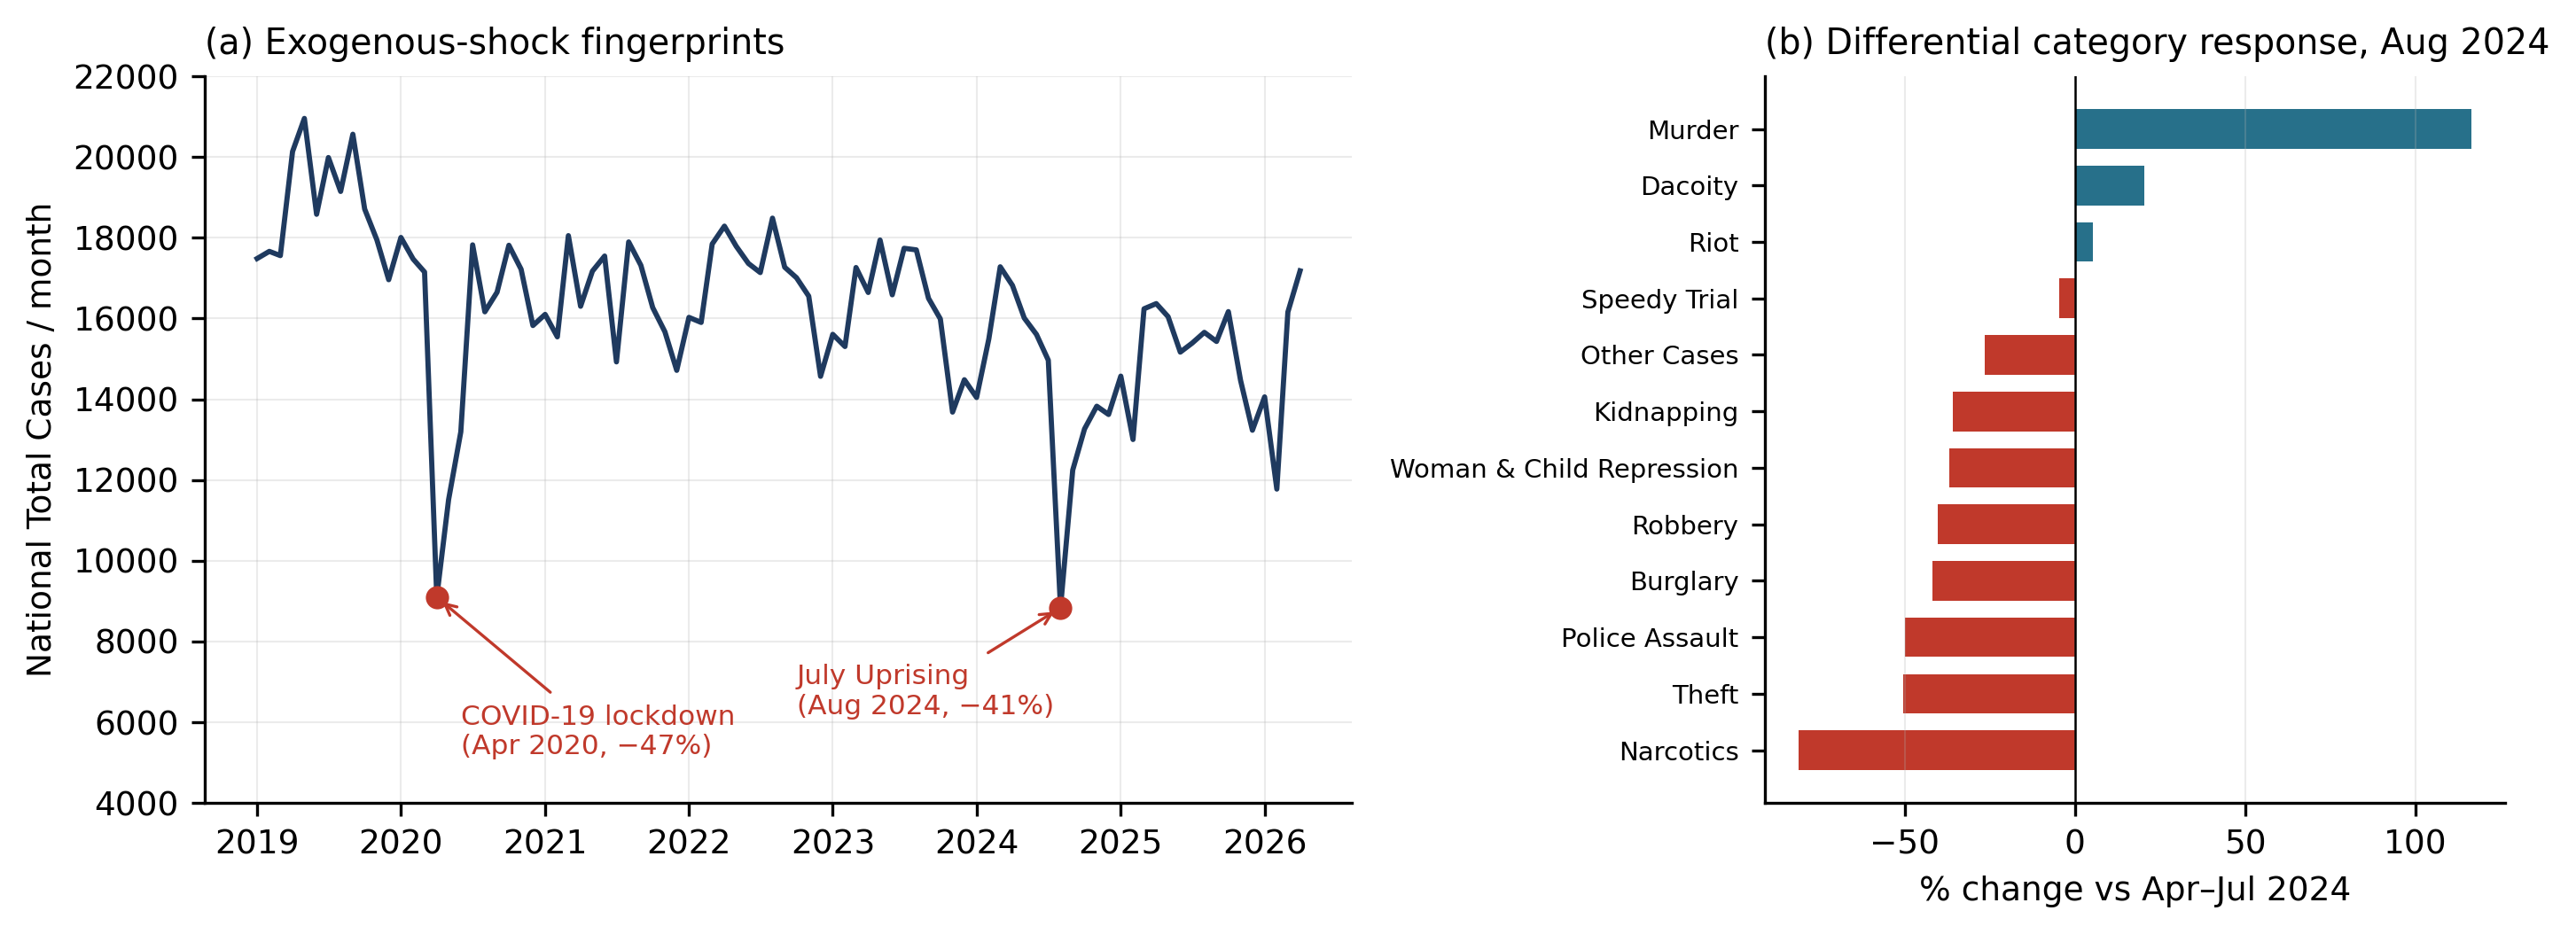
\includegraphics[width=\columnwidth]{figures/fig_data_authenticity.png}
\caption{External-consistency checks on the PHQ series. (a) National monthly Total Cases, with the
two documented nationwide disruptions (the 2020 public-health restrictions and the August 2024
transition) marked. (b) Category-level change in August 2024 relative to the April--July 2024
average: the response is heterogeneous rather than a uniform shift, consistent with genuine
event-driven recording rather than routine re-entry of prior figures.}
\label{fig:validity}
\end{figure}

\section{Methodology}
\subsection{Definitions and Evaluation Conventions}
\label{sec:terms}
We use the following conventions throughout. The \emph{forecast horizon} is the number of months
ahead predicted; we report horizons of 1, 3, 6, and 12 months. \emph{Rolling-origin validation}
repeatedly fits the model on an expanding window, forecasts the next $h$ months, advances the
origin, and repeats, so that every evaluation point lies strictly after its training window. A
\emph{post-release back-test} fixes the origin at a past date (April 2025), forecasts forward, and
compares the result against PHQ figures published only later. In both protocols, no information
dated after the forecast origin enters training or model selection, which avoids look-ahead
leakage. For readability we report \emph{practical accuracy} as $100-\mathrm{MAPE}$ (a 7\% mean
absolute percentage error reads as 93\% practical accuracy); MAPE and MASE remain the underlying
error measures.

\subsection{Forecasting Models}
We use a transparent set of seven forecasting models, plus an ensemble (a simple average of ETS,
Theta, ARIMA, SARIMA, and LightGBM). Every model is standard and easy to inspect:
\begin{itemize}
  \item \textbf{Naive} and \textbf{Seasonal Naive}: simple baselines (repeat the last value, or
        the value from the same month last year).
  \item \textbf{ETS}, \textbf{Theta}, \textbf{ARIMA}, \textbf{SARIMA}: classical time-series
        models that capture trend and yearly seasonality.
  \item \textbf{LightGBM}: a gradient-boosted tree using past months as features.
  \item \textbf{Ensemble}: the average of ETS, Theta, ARIMA, SARIMA, and LightGBM. Averaging
        reduces the risk of any single model going wrong.
\end{itemize}
If a model ever produces a broken or unrealistic number (non-finite, negative, or implausibly
large), the system automatically falls back to the Seasonal Naive forecast and records the event
in a persistent audit log. This guard runs identically in the analysis notebook and in the
monitoring software, so that a single failed fit cannot silently corrupt the results.

\subsection{Validation and Back-Testing Protocol}
We tested in two ways that support each other:
\begin{itemize}
  \item \textbf{Rolling-origin validation} over the full data, at horizons of 1, 3, 6, and 12
        months, using an expanding training window.
  \item \textbf{A fixed back-test:} we trained only on January 2019 to April 2025, then forecast
        1, 3, 6, and 12 months ahead, landing on May 2025, July 2025, October 2025, and April 2026. We compared
        each forecast with the real, later-released PHQ number for that month.
\end{itemize}
We group the crime types into \emph{stable} types (Total Cases, Murder, Theft, Woman \& Child
Repression, Robbery), which have large, steady monthly counts, and \emph{hard} types (Narcotics
recovery, Kidnapping, Dacoity), whose counts are small and jumpy. Our headline accuracy uses the
stable types only (Section~\ref{sec:xai}).

\section{Results}
\label{sec:results}
We report two separate evaluations: (A) the fixed back-test of the April 2025
forecast, and (B) the rolling-origin validation over all the data.

\subsection{Post-Release Back-Test of the April 2025 Forecast}
This is the most direct out-of-sample evidence we report. We made a forecast in April 2025, using \emph{only}
data up to that point, and then checked it against the real PHQ numbers that came out later. This is a single forecast origin for one series, national Total Cases. The ensemble forecast was:
\begin{itemize}
  \item \textbf{98.9\%} accurate 1 month ahead (May 2025),
  \item \textbf{97.8\%} accurate 3 months ahead (July 2025),
  \item \textbf{92.8\%} accurate 6 months ahead (October 2025),
  \item \textbf{86.1\%} accurate 12 months ahead (April 2026).
\end{itemize}
All four figures are for national Total Cases at this single April 2025 origin, not the rolling-origin averages over the five stable crime types in Table~\ref{tab:horizon} (where the 12-month figure is 89.9\%). A single national total swings more than an average over stable series, so its long-horizon accuracy is naturally a little lower; the two are measured differently and reported separately.
Fig.~\ref{fig:backtest} shows the full picture: the dark line is the real, verified history; the
dashed line is the April 2025 forecast; and the marked points are the four checks. The forecast
stays close to reality, and accuracy is naturally highest at the short horizon and slowly drops as
we look further ahead, as expected for a well-specified forecast. Part of this short-horizon accuracy reflects the strong monthly seasonality and persistence in crime counts, not model skill alone. This same checking step
is built into the monitoring loop (Section~\ref{sec:monitoring}): every new month becomes a fresh
test of the last forecast.

\begin{figure}[t]
\centering
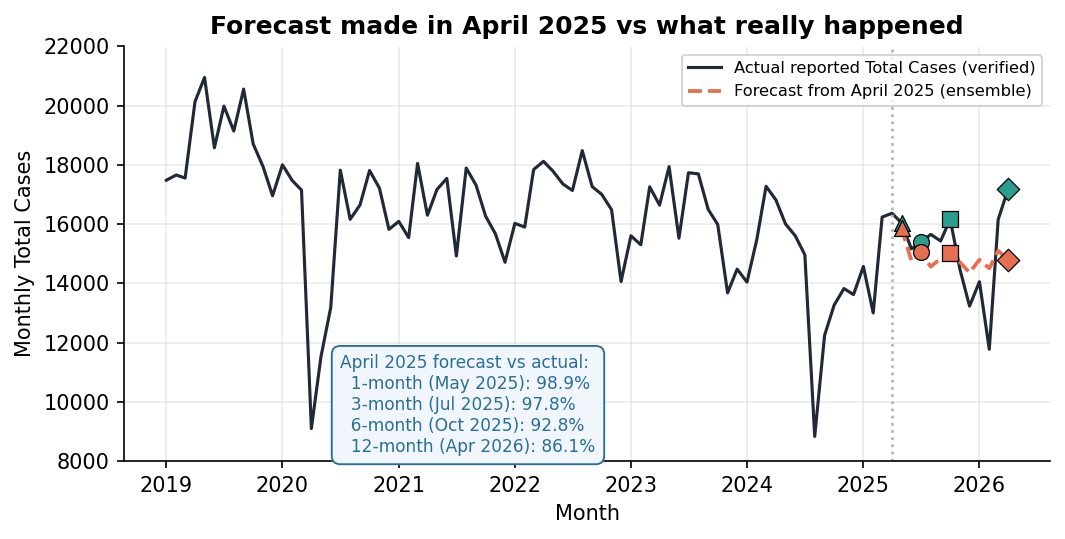
\includegraphics[width=\columnwidth]{figures/fig1_backtest_3horizon.png}
\caption{The forecast made in April 2025 versus the real PHQ numbers released later (national
Total Cases, single origin). The forecast tracks reality closely: 98.9\% accurate at 1 month,
97.8\% at 3 months, 92.8\% at 6 months, and 86.1\% at 12 months. This is a fair test: the model
never saw any data after April 2025.}
\label{fig:backtest}
\end{figure}

\subsection{Rolling-Origin Validation}
The repeated rolling-origin test agrees with the back-test. Unlike the single-origin back-test
above, these numbers are averaged over many forecast origins and over the five stable crime types,
so they are not expected to match the back-test figure for any single month; the two tests are
complementary, not contradictory. For the stable crime types, the average
error stays low at every horizon, well under the 18\% line (82\% accuracy) that we treat as the
minimum bar (Table~\ref{tab:horizon}, Fig.~\ref{fig:horizon}). Using a ``furthest horizon that
still passes'' rule, the 12-month horizon (89.9\% accuracy) is our headline, while the 1-month
horizon is the most accurate at 94.7\%.

\begin{table}[t]
\caption{Rolling-origin accuracy for stable crime types, by horizon.}
\label{tab:horizon}
\centering
\renewcommand{\arraystretch}{1.2}
\begin{tabular}{@{}ccccc@{}}
\toprule
\textbf{Horizon} & \textbf{MAPE (\%)} & \textbf{Practical acc. (\%)} & \textbf{MASE} & \textbf{Status} \\
\midrule
1  & 5.27  & 94.7 & 0.346 & pass \\
3  & 7.34  & 92.7 & 0.500 & pass \\
6  & 8.33  & 91.7 & 0.544 & pass \\
12 & 10.13 & 89.9 & 0.674 & pass (headline) \\
\bottomrule
\end{tabular}
\end{table}

\begin{figure}[t]
\centering
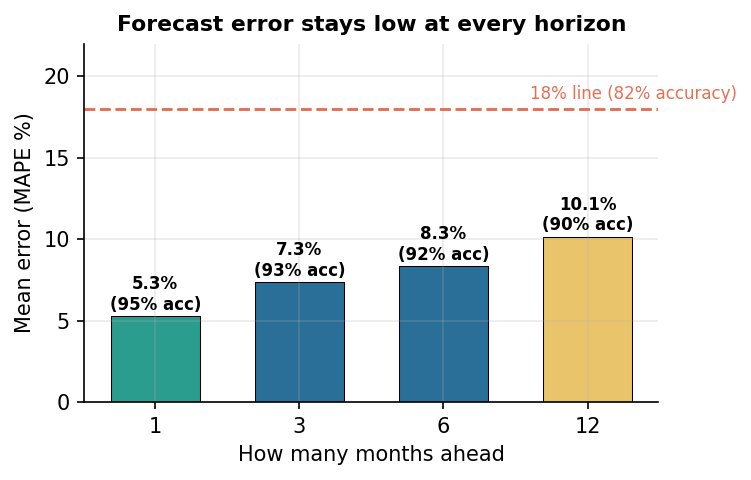
\includegraphics[width=\columnwidth]{figures/fig2_horizon_mape.png}
\caption{Average error for stable crime types at each horizon. Every bar stays below the 18\% line
(82\% accuracy), which is why we can stand behind a 12-month forecast, not just a 1-month one.}
\label{fig:horizon}
\end{figure}

The ensemble was the most reliable model overall, with the lowest average error and beating the
Seasonal Naive baseline in 75\% of the test cases (Table~\ref{tab:model}, Fig.~\ref{fig:model}).
A MASE below 1.0 means a model beats the seasonal baseline on average; the ensemble reaches 0.577,
and every classical model here is below 1.0.
LightGBM was not competitive on this short monthly history, which is expected: tree models need
more data than we have.

\begin{table}[t]
\caption{Model comparison over stable crime types (lower error is better).}
\label{tab:model}
\centering
\renewcommand{\arraystretch}{1.2}
\begin{tabular}{@{}lccc@{}}
\toprule
\textbf{Model} & \textbf{Mean MAPE (\%)} & \textbf{Mean MASE} & \textbf{Beats Seasonal Naive (\%)} \\
\midrule
\textbf{Ensemble} & \textbf{8.96} & \textbf{0.577} & \textbf{75} \\
ETS      & 9.64  & 0.633 & 55 \\
Seasonal Naive & 9.84 & 0.636 & n/a \\
Theta    & 10.19 & 0.670 & 55 \\
SARIMA   & 10.23 & 0.672 & 20 \\
ARIMA    & 10.63 & 0.702 & 45 \\
Naive    & 12.35 & 0.819 & 15 \\
LightGBM & 14.82 & 0.890 & 25 \\
\bottomrule
\end{tabular}
\end{table}

\begin{figure}[t]
\centering
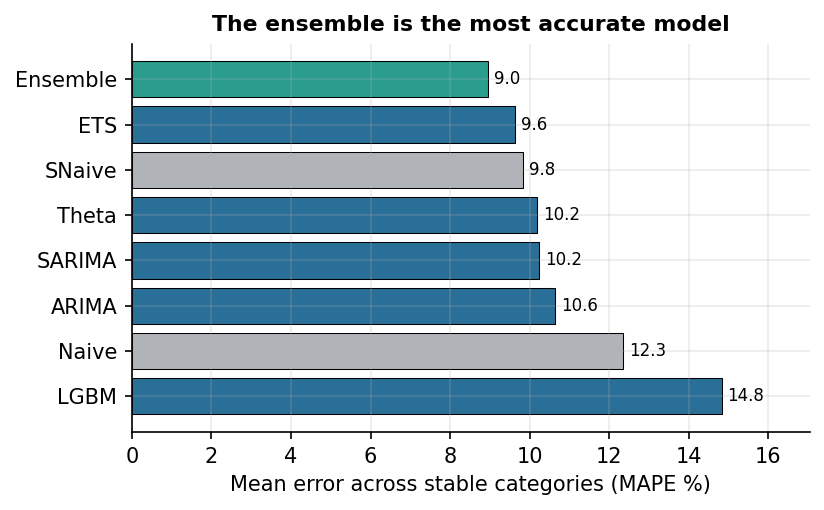
\includegraphics[width=\columnwidth]{figures/fig3_model_comparison.png}
\caption{Average error by model across stable crime types. The ensemble (green) is the most
accurate. Tree-based LightGBM trails because the monthly history is short.}
\label{fig:model}
\end{figure}

\subsection{Scenario Projection to December 2027}
Using all 88 verified months, we extend the ensemble forecast to December 2027
(Fig.~\ref{fig:scenario}). \textbf{These numbers are a planning scenario, not a verified
prediction.} We attach no accuracy claim to them. They are useful for rough planning, and the
shaded band is a reminder that the real values will differ.

For concreteness, the scenario keeps national monthly Total Cases roughly in the 14{,}600 to 16{,}600 range through 2027, ending near 14{,}600 in December 2027, for an implied 2027 total of about 184{,}000 cases (Table~\ref{tab:scenario}). These remain planning figures with no accuracy claim.

\begin{table}[t]
\caption{Scenario projection for national Total Cases (planning only; no validated accuracy claim). Horizons are measured from the last observed month, April 2026.}
\label{tab:scenario}
\centering
\begin{tabular}{@{}llr@{}}
\toprule
Horizon & Target month & Projected Total Cases \\
\midrule
+1 month & May 2026 & 16{,}639 \\
+3 months & July 2026 & 16{,}118 \\
+6 months & October 2026 & 15{,}352 \\
+12 months & April 2027 & 16{,}142 \\
+20 months & December 2027 & 14{,}587 \\
\bottomrule
\end{tabular}
\end{table}

\begin{figure}[t]
\centering
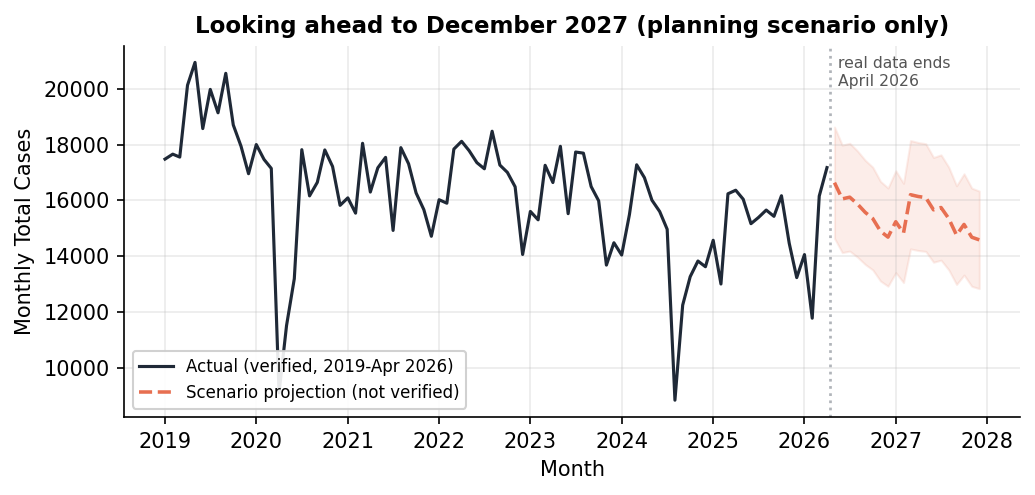
\includegraphics[width=\columnwidth]{figures/fig4_scenario_dec2027.png}
\caption{Verified history (to April 2026) with a planning-only projection to December 2027. The
vertical line marks where real data ends. No accuracy is claimed for the projected part.}
\label{fig:scenario}
\end{figure}

\section{Explainability and Error Analysis}
\label{sec:xai}
We add a diagnostic interpretability layer that leaves the models and the reported accuracy
unchanged; it characterizes what the forecaster relies on and where its errors concentrate.

\subsection{Feature Importance}
We trained a LightGBM model on the same past-month features the pipeline uses and read both its
built-in importance and a model-agnostic permutation check~\cite{breiman2001}. Both point the same
way (Fig.~\ref{fig:perm}):
\begin{itemize}
  \item the \textbf{most recent month} matters most;
  \item the \textbf{recent ups and downs} (how bumpy the last few months were) matter next;
  \item the \textbf{month of the year} matters too, which fits the yearly pattern in crime data.
\end{itemize}
The agreement between the two methods indicates that the model relies on recent
level and seasonality rather than noise.

\begin{figure}[t]
\centering
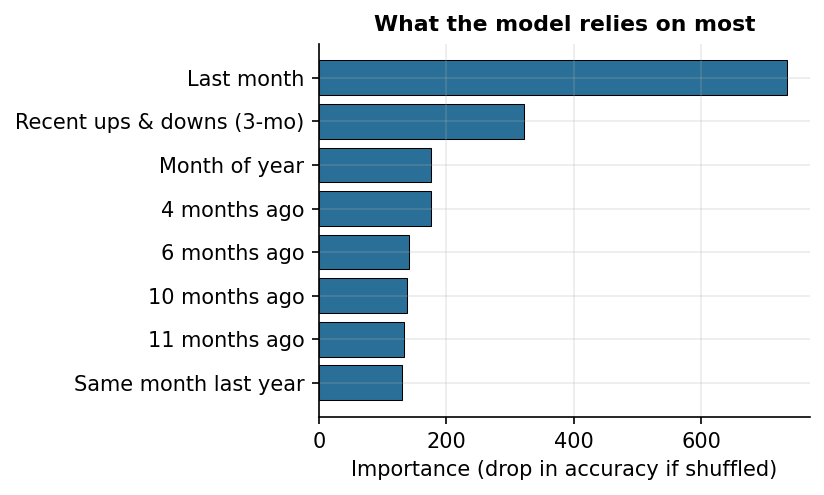
\includegraphics[width=\columnwidth]{figures/fig5_permutation_importance.png}
\caption{What the model relies on most, measured by how much accuracy drops when each input is
shuffled. The last month and recent movement lead, with month-of-year close behind, which is sensible,
not noise.}
\label{fig:perm}
\end{figure}

\subsection{Error by Crime Category}
We also measured the error for each crime type (Fig.~\ref{fig:err}). Two clear patterns appear:
\begin{itemize}
  \item \textbf{Stable types} (Theft at 6.4\% error, Total Cases at 7.0\%, Murder at 8.6\%) are
        easy to forecast because their monthly counts are large and steady.
  \item \textbf{Hard types} (Kidnapping at 22\%, Dacoity at 18\%) are difficult because their counts
        are small, so even a swing of a few cases looks like a big percentage error.
\end{itemize}
This is why the headline accuracy is reported on the stable types, with the hard types reported
separately rather than folded into the headline figure.

\begin{figure}[t]
\centering
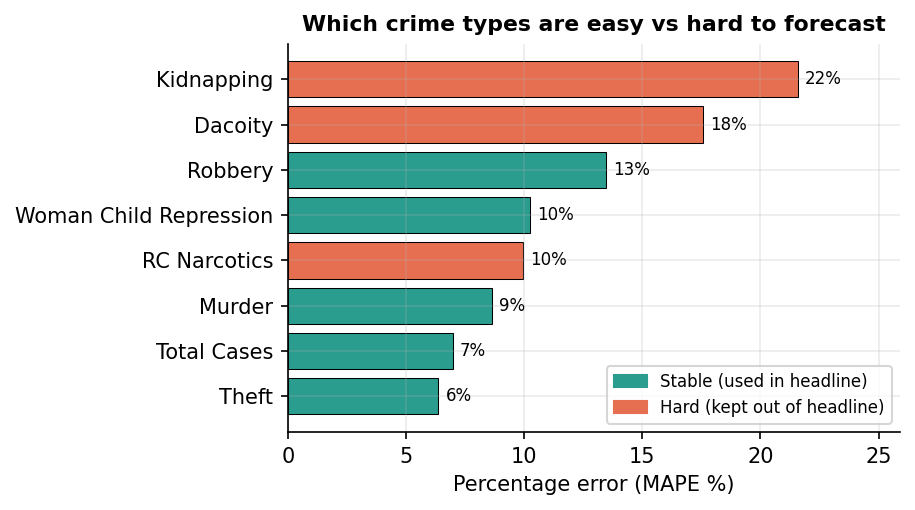
\includegraphics[width=\columnwidth]{figures/fig6_error_contribution.png}
\caption{Percentage error by crime type. Green types are stable and used in the headline; orange
types are hard (small, jumpy counts) and kept separate. The split is reported openly.}
\label{fig:err}
\end{figure}

\subsection{Scope of the Explainability Layer}
The explanation layer is a diagnostic, not a cause. It shows what the model leans on; it does not
prove that crime in the real world works that way. It shows where forecasts miss; it does not
explain why crime itself went up or down. It changes none of the accuracy numbers above.

\section{Operational Monitoring System}
\label{sec:monitoring}
We implemented the framework as a deployable application so it can run as a monthly routine inside
a police or planning office. Fig.~\ref{fig:workflow} shows the loop; the application:
\begin{itemize}
  \item \textbf{Adds a new month} from a CSV or Excel file, and checks it automatically (missing
        units, missing crime types, or impossible values are flagged before anything is saved).
  \item \textbf{Re-checks the last forecast} against the new real numbers, so accuracy is tracked
        as it happens.
  \item \textbf{Retrains the models} on the updated data and produces the next forecast.
  \item \textbf{Watches for drift}: if accuracy starts slipping, it raises a warning and
        recommends recalibration.
  \item \textbf{Shows the explanation views} (which inputs matter, which crime types are hard).
  \item \textbf{Controls access by role} (administrator, operator, reviewer, viewer), so data entry
        and approval are separated.
\end{itemize}
The application keeps a full audit trail (who added or approved what, and when), stores every
forecast so it can be scored later, and writes any model fallback to that same persistent audit
log. It was checked with an automated smoke-test suite of 18 checks across seven groups: seed-data
integrity, duplicate-month safety, forecasting completion, recalibration persistence,
forecast-vs-actual lookup, restart-safe database reads, and role-based authentication; all 18 pass.
It is straightforward to deploy on a single office machine or a small server.

\begin{figure}[t]
\centering
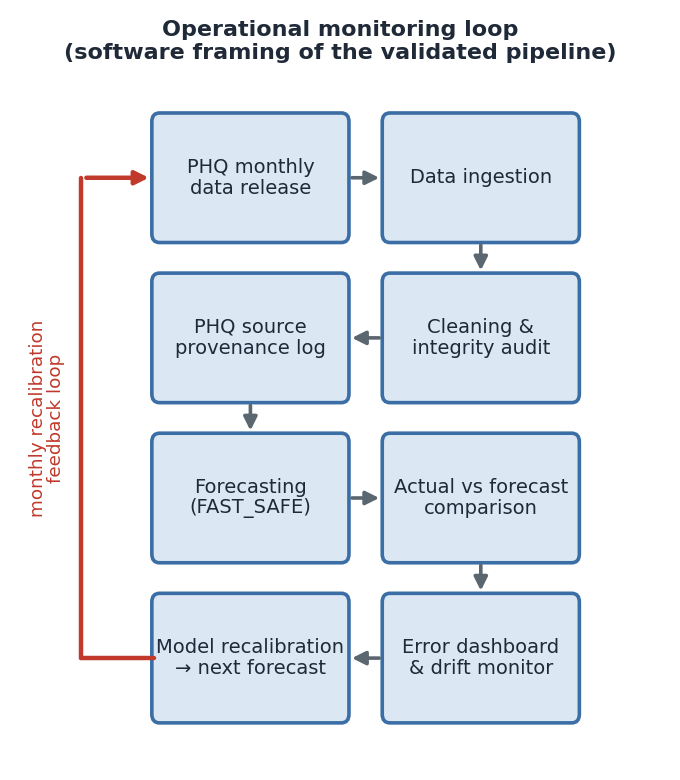
\includegraphics[width=\columnwidth]{figures/fig7_workflow.png}
\caption{The monthly monitoring loop. Each new PHQ release is added and checked, the previous
forecast is scored against it, drift is watched, the models are retrained, and the next forecast is
produced, then the cycle repeats.}
\label{fig:workflow}
\end{figure}

\section{Limitations}
\label{sec:limitations}
Several boundaries apply. The system forecasts reported crime---incidents recorded and published by
PHQ---and therefore does not capture unreported crime, nor does it predict individual offenders or
specific locations; its unit of analysis is the monthly count. The history is short (88 months),
which is why classical models and their ensemble outperform heavier deep-learning architectures
here. Accuracy decays with horizon, so short-range forecasts are stronger than long-range ones, and
the forward projection is a planning scenario rather than a validated forecast. Finally, the series
is subject to abrupt exogenous shocks---such as the 2020 pandemic restrictions and the August 2024
political transition, both visible in the data---that no statistical model can anticipate; the
monitoring loop is designed to detect and adapt to such breaks after they occur rather than to
predict them.

\section{Future Work}
\begin{itemize}
  \item Add external covariates (for example population or economic indicators) under the same
        source-checking and back-testing rules.
  \item Add district-level forecasting under the same checking and testing rules.
  \item Explore privacy-preserving federated learning~\cite{mcmahan2017fl,kairouz2021fl} so multiple
        police units could improve a shared model without sharing raw records.
  \item Add automatic alerts (email or dashboard) when drift crosses the warning level.
\end{itemize}

\section{Conclusion}
We presented an end-to-end framework that takes source-verified PHQ data, forecasts reported-crime
counts under leakage-free evaluation, and runs as a monthly monitoring application. In a
post-release back-test, an ensemble of classical models trained only on data through April 2025
forecast national Total Cases at 98.9\%, 97.8\%, 92.8\%, and 86.1\% practical accuracy at horizons
of 1, 3, 6, and 12 months, and was the most reliable model overall. Stable and hard-to-forecast
categories are reported separately, an interpretability layer exposes the drivers of forecast
error, and the accompanying software supports continued operational use. Forward projections are
planning scenarios only. Applied within these bounds, the framework offers a reproducible basis for
anticipating movements in Bangladesh's official crime statistics and for monitoring forecast
quality as new data arrives.

\section*{Reproducibility}
The verified dataset~\cite{dataset_repo}, the analysis notebook with all results and figures, and
the monitoring application~\cite{software_repo} are provided as public companion repositories, so
every number and figure in this paper can be regenerated.

\bibliographystyle{ieeetr}
\bibliography{references}

\end{document}
